
\documentclass[a4paper,12px,twocolumn]{article}
\usepackage{ragged2e}
\usepackage[margin=1in]{geometry}
\usepackage{graphicx}
\usepackage{color}
\graphicspath{ {./images/} }

\usepackage{multicol}
\setlength{\columnsep}{1cm}

\begin{document}
\begin{flushleft}
\section{Introduction}
\justifying{
The Fourier transform is used to assess geometric characteristics of a particular spatial
image domain. An image's representation in the Fourier domain is a representation the number
of basis sine and cosine functions of varying frequencies which are present in the image. Because
the image in the Fourier domain is decomposed into into its sinusouidal components, it is easy to
examine the frequencies of the image and their geometric relation.

This report explains my process of classification of text based on features of the
image extracted from the Fourier domain.
}
\section{Approach to analysis in the Fourier domain}


To start with, I superimposed the magnitude spectrums of the training data to produce
three graphs which illustrate the geometric characteristics of the letters in the Fourier
space. Over the top I have illustrated the regions of the chosen features by blue lines,
the feature selection process is detailed in section 3

\begin{figure}[h!]
  \caption{Fourier transform of T characters}
  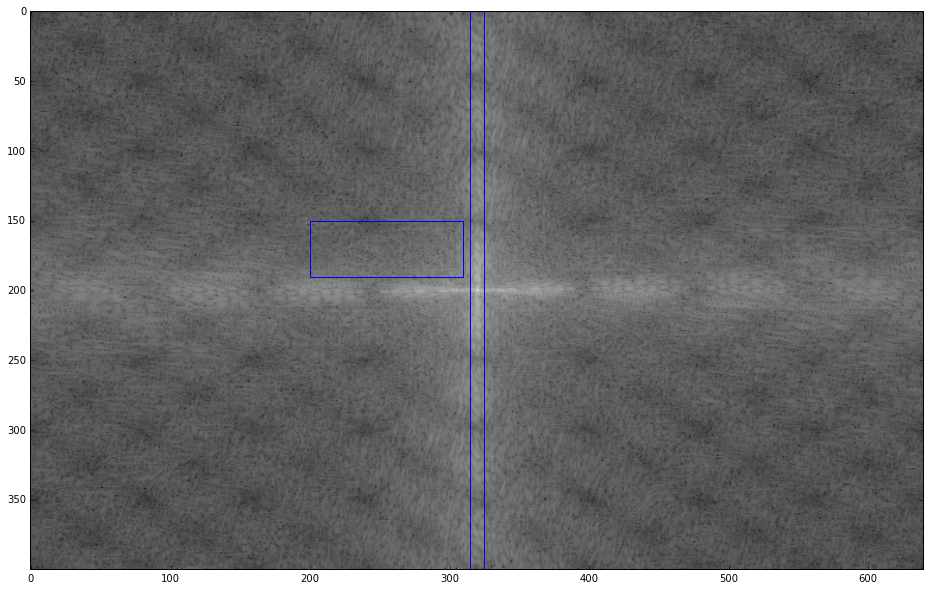
\includegraphics[scale=0.25]{fourierT}
\end{figure}

\begin{figure}[h!]
  \caption{Fourier transform of S characters}
  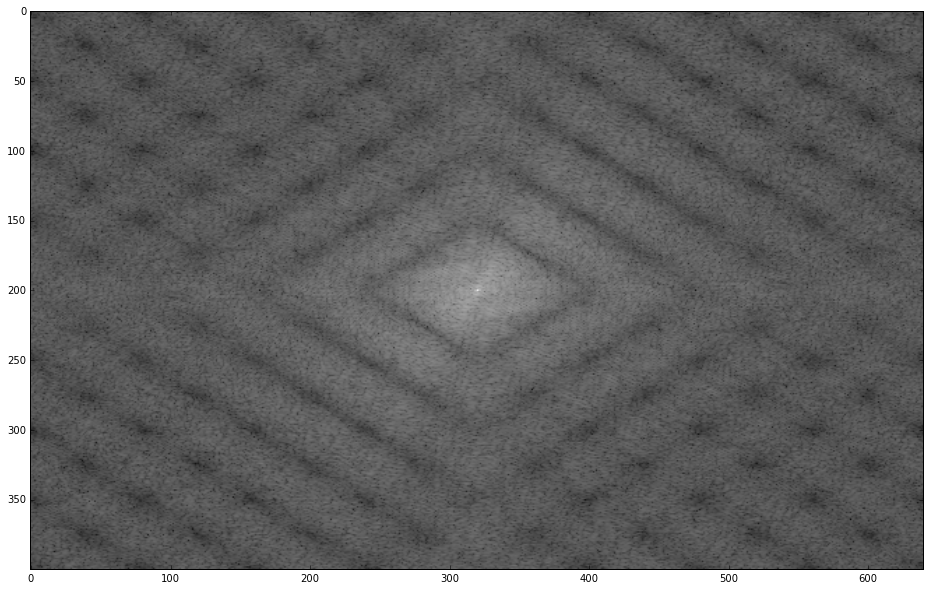
\includegraphics[scale=0.25]{fourierS}
\end{figure}

\begin{figure}[h!]
  \caption{Fourier transform of V characters}
  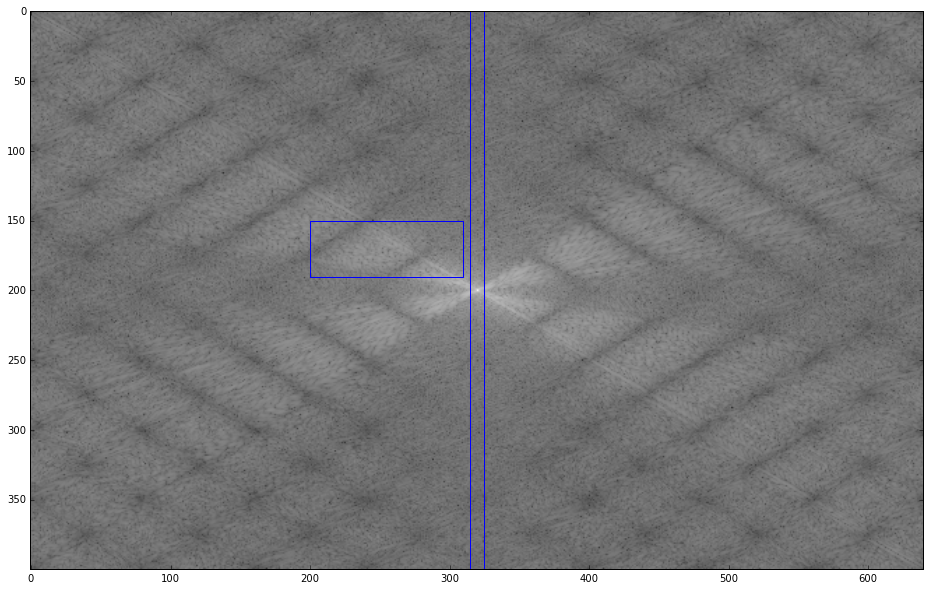
\includegraphics[scale=0.25]{fourierV}
\end{figure}




\smallskip

Considering the three Fourier images

\justifying{
\begin{itemize}
    \item Figure 1 shows the general fourier space for the character T, from the image we
    can observe that the power spectrum has high magnitude along the vertical bar passing through the centre,
    this corresponds to the line which forms the top of a character T. Similarly, there is another high magnitude bar passing horizontally
    through the centre, corresponding to the vertical part of the character

    \item Figure 2 shows the general fourier space for the character S, the power spectrum for S shows only small magnitudes for directions
    in exclusively the horizontal or vertical direction, this corresponds to the fact that a regular character S does not change in only
    the vertical or horizontal directions. As seen, the highest magnitudes lie relatively evenly distributed within the central diamond
    region, illustrative of change in both the horizontal and vertical directions, at varying angles. It is also just visible with the naked eye
    that there is a slightly more intense band in the $u=v$ line of the fourier space, this corresponds to the almost diagonal line which is part
    of some of the S test characters

    \item Figure 3 shows the general fourier space for the character V, the power spectrum shows two distinct bands in the lines $u = v$ and $u=-v$,
    these correspond to the two diagonal lines which form the letter V. We can also see the magnitude along vertical line
    passing through the centre is very low, the corresponds to the fact that there is very little change purely in the horizontal direction for the
    character V, eg the only point at which exclusively horizontal change is likely to occur is at the bottom of the character

\end{itemize}
}

\section{Feature extraction}
\justifying{
    The characters are classified into three seperate classes using two features, each feature is designed to positvely identify one character,
    the third character is indentified by logical deduction. The features are obtained by taking the sum of the square of the magnitude in specific
    regions as shown in figures 1 to 3.

    \smallskip

    the first feature I picked was a narrow vertical rectangle passing through the centre and spanning the height of the image, I reasoned that
    the rectangle would measure change only in the horizontal direction of a image, consequently this feature should produce the
    highest value for for T, with a lower value for S, as S contains some horizontal information in the top and bottom parts of the character,
    and the lowest magnitude for V, as there is only a very small area at the bottom in which the change
    is purely horizontal.


    \smallskip

    The second feature chosen was a rectangular box in the top left quadrant of the image as shown, this area is aimed at positively identifying
    the character V. I reasoned that this feature should have the highest value for this character owing to the fact that the character
    V changes most in both the horizontal and vertical directions.


    % I reasoned that
    % I should use a feature which did not include change in the vertical or horizontal directly exclusively.
    % I reasoned that the T would have the lowest power magnitude in the region mentioned, owing to the fact that a T
    % is composed of a vertical and horizontal line placed orthogonally to one another. The next highest magnitude should
    % be that of the S, as seen from the Fourier space, S has a high magnitude in the central diamond region. V should have
    % the highest magnitude owing to the fact it changes the most in both the horizontal and vertical directions
}

\section{Results of Fourier Domain analysis and analysis of the classifier}

    Using the features chosen in the previous section, I computed the sum of the power spectrum in the regions selected
    by the features for each letter. I then applied the nearest neighbour procedure with $k=1$ and uniform weighting to the list of
    values produced by the feature extraction, the results are shown in figure 4. The figure shows the decision regions for the
    nearest neighbour classification given a test point, the \textcolor{red}{red} region shows the area where a point will be classified as a T,
    the \textcolor{blue}{blue} region shows where a point will be classified as a S, and the \textcolor{green}{green} area shows where a point will be classified
    as a V.



    \begin{figure}[h!]
      \caption{Result of feature extraction, with decision boundaries shown}
      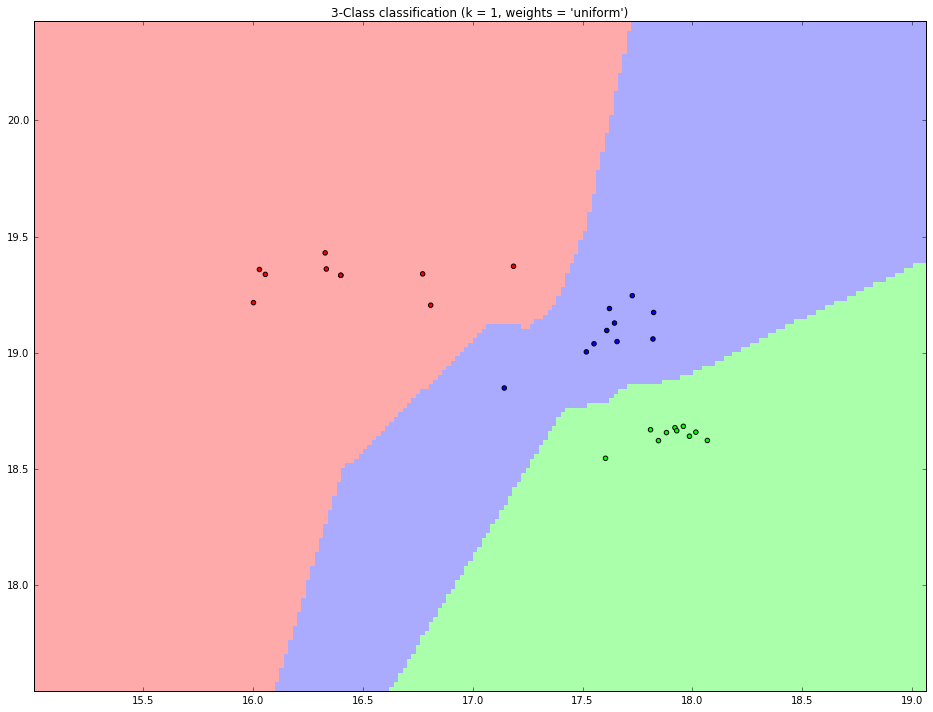
\includegraphics[scale=0.25]{decision}
    \end{figure}



    The training data produced three regions which correspond to the letters T, V and S. The clustering seems satisfactory, except for
    one of the S points. Observing figure 4 we can see that one S value is far closer to the V decision boundary than the rest.
    I reasoned that the shift towards the V decision boundary must relate to a test character which had lower overall magnitude in the
    center vertical line of its Fourier space. Further this character would have a lower magnitude in diagonal lines of its Fourier space.
    One by one I removed datapoints from the dataset and plotted the resulting nearest neighbour classification, I found that the point to be \textbf{S7}.
    The lines forming S7 were thicker than all the other test Ss, furthermore, it was more curved at its top and bottom.
    As the top and bottom of the S were not as straight as the others, their respective magnitudes as computed by the vertical rectangle feature
    was lower, hence why it is shifted towards the S/V decision boundary.

    \bigskip
    \justifying{
    To test my classifier, I created 10 new images for each character. The figure 5 shows the resulting classification for the points. Observing the graph
    we can see that all input Ts have been classified correctly, each T also lies relatively far way from the decision boundary between T and S. Considering
    the next character, Ss have all also been classified correctly for my test data, some of the Ss are near the S/V decision boundary, this corresponds
    to a test S which had a particularly diagonal middle section. My classifier classifier also correctly identified all test V characters.
    }
    \begin{figure}[h!]
      \caption{Result of feature extraction, with test data points shown}
      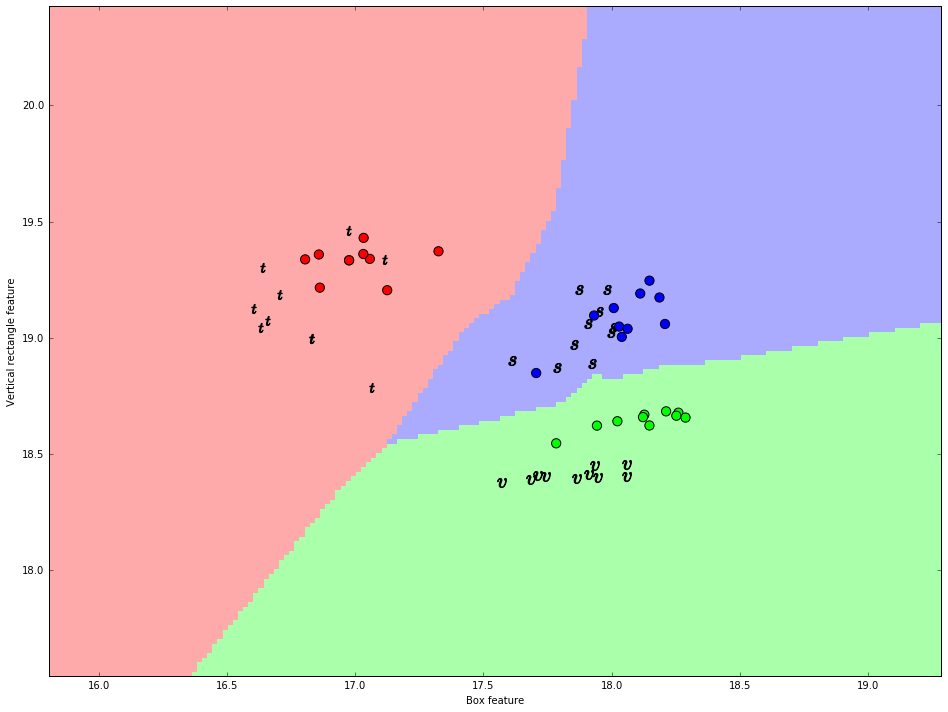
\includegraphics[scale=0.25]{testpoints}
    \end{figure}

    \bigskip
    \justifying{

    Next, I wanted to see how the classifier would cope with extreme cases for some test characters. I created the characters seen,
    the characters seen have been drawn to any weaknesses in the chosen features. Figure 6 illustrates the resulting classification for
    these points
    }

    \bigskip
\begin{figure}[h!]
        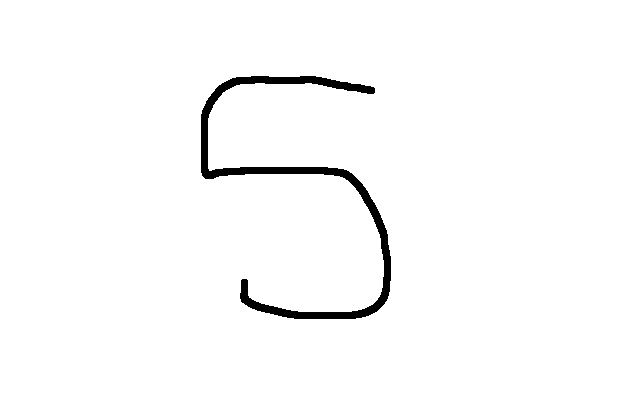
\includegraphics[scale=0.1]{tS11}
        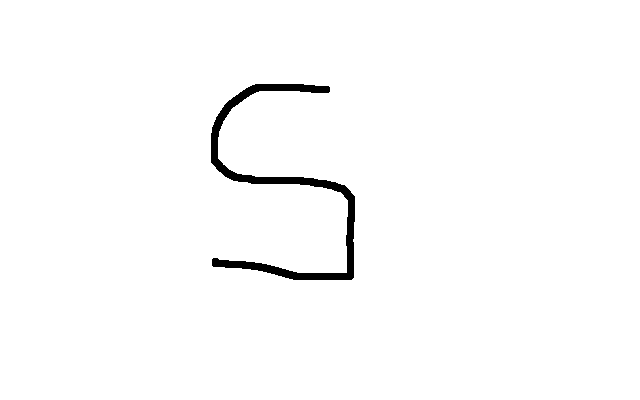
\includegraphics[scale=0.1]{tS12}
        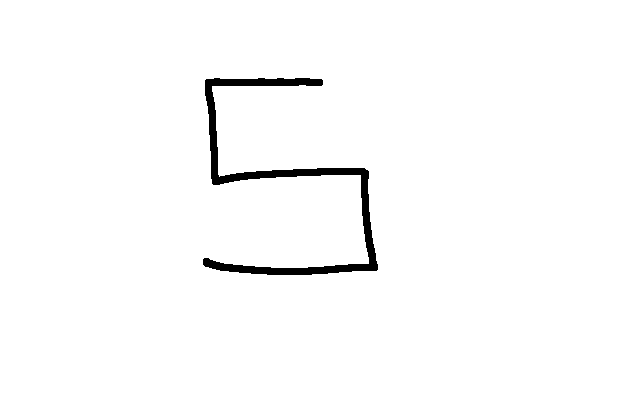
\includegraphics[scale=0.1]{tS13}
        \includegraphics[scale=0.1]{tv11}
        \includegraphics[scale=0.1]{tv12}
        \includegraphics[scale=0.1]{tv13}
        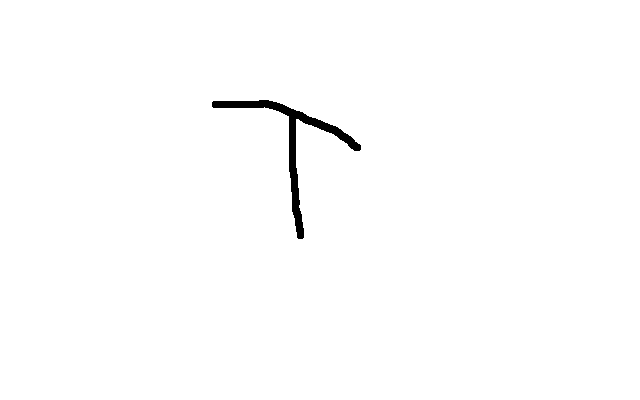
\includegraphics[scale=0.1]{tT11}
        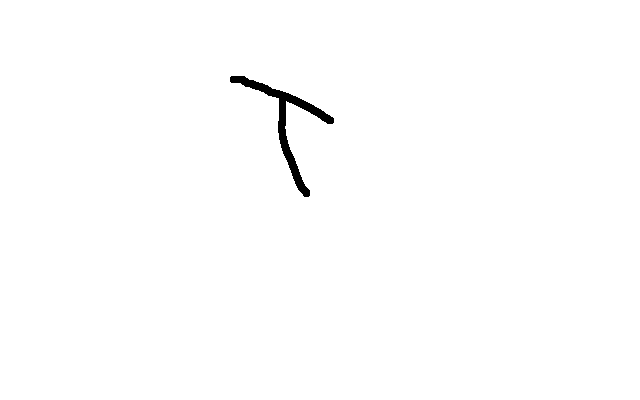
\includegraphics[scale=0.1]{tT13}
        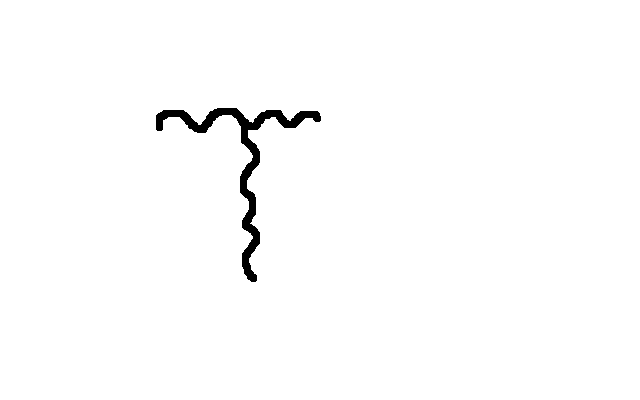
\includegraphics[scale=0.1]{tT12}
    \end{figure}

        \begin{figure}[h!]
          \caption{Assignment of extreme test characters}
          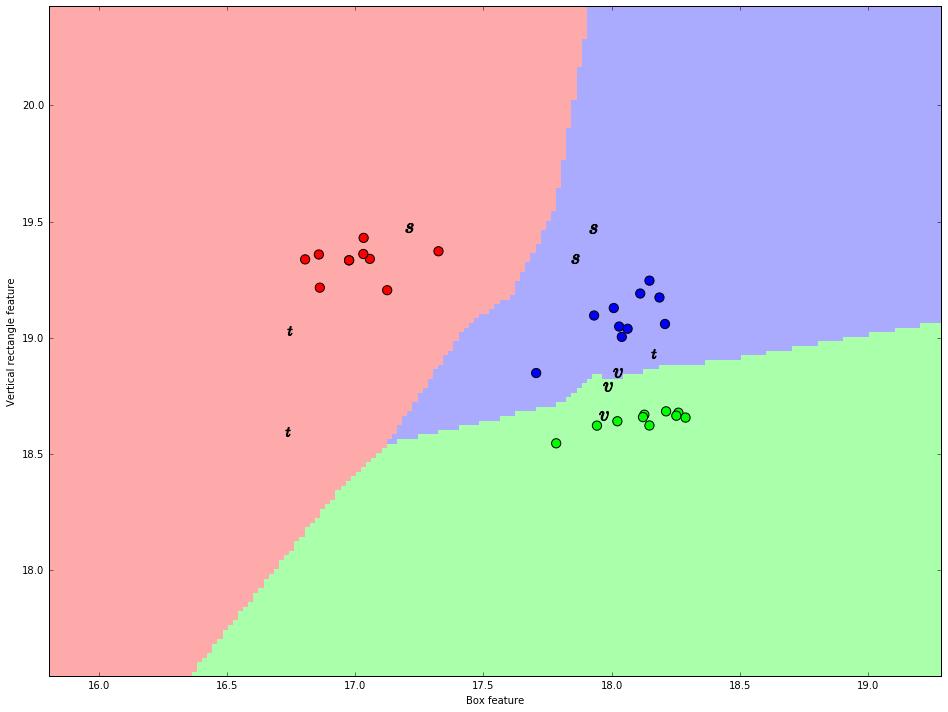
\includegraphics[scale=0.25]{extremechars}
        \end{figure}

    \justifying{

        figure 6 shows the resulting assignment of the characters seen above. Referring first to the Ss,
        observing the figure we can see that the first two Ss have been classified correctly  despite the fact that both contain
        areas of exclusive horizontal change, the small amount of curvature was enough to distinguish them from Ts. The third S, however,
        has areas almost \textit{only} containing exclusive horizontal or vertical change, leading to its classification as a T


        \smallskip

        Considering the Ts, observing the figure we can see that two of them have been correctly classified as Ts, the points lie further
        away from the training cluster due to the fact that the Ts drawn have a much smaller horizontal component as a whole. The T composed
        of wiggly lines has been classifed as an S owing to its change magnitude in many directions.

        \smallskip
        Lastly considering the Vs, we can see from the figure that again two of them have been correctly classified, they lie very close
        to the boundary because they contain enough horizontal change to push them in the direction of T by the vertical box feature. This argument
        applies to why the third v is incorrectly classified as an S - the box classifier identifies it as a V, but because of the presence of
        the horizontal line, it is shifted by the first feature in the T direction, hence it is classified as an S.


    }



% \section{Analysis of the classifier}

% \section{Decision region plots and their angles}


\section{Classification of A and B}

\justify{
Figure 6 shows the classification of the characters A and B, as seen both
lie near the centre of the S decision area, hence both have been classified
as Ss. This can be explained by examining their Fourier spaces.
}


\begin{figure}[h!]
  \caption{Classification of A and B}
  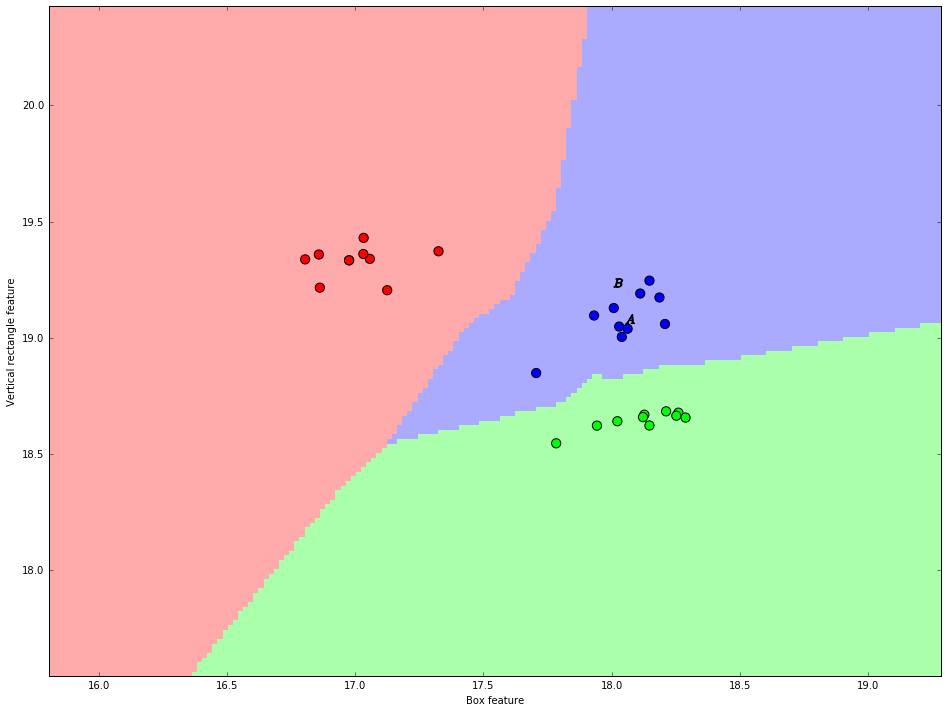
\includegraphics[scale=0.25]{AB}
\end{figure}

\justify{
    Why is A classified as an S? We can see why A has been classified this
    way if we examine the classification feature by feature. Firstly, considering the box feature:
    A lies almost directly in the centre of the V cluster with respect to the box feature axis.
    This can be explained by the diagonals seen in the fourier space of the letter A as seen in figure 8 - these cause
    the box feature to classify the character as a V. Secondly, examining the classification based on the
    vertical rectangle feature: the vertical rectangle feature is sensitive to horizontal change. Again
    examining the Fourier space of the A, we can see a line of high magnitude running almost through
    the centre, this corresponds the the horizontal part of the character A. Hence because of
    this component, the vertical rectangle feature classifies this as a T. So, overall the A is classified
    as an s because of the combination of these two features.
}
\begin{figure}[h!]
  \caption{Fourier space of A}
  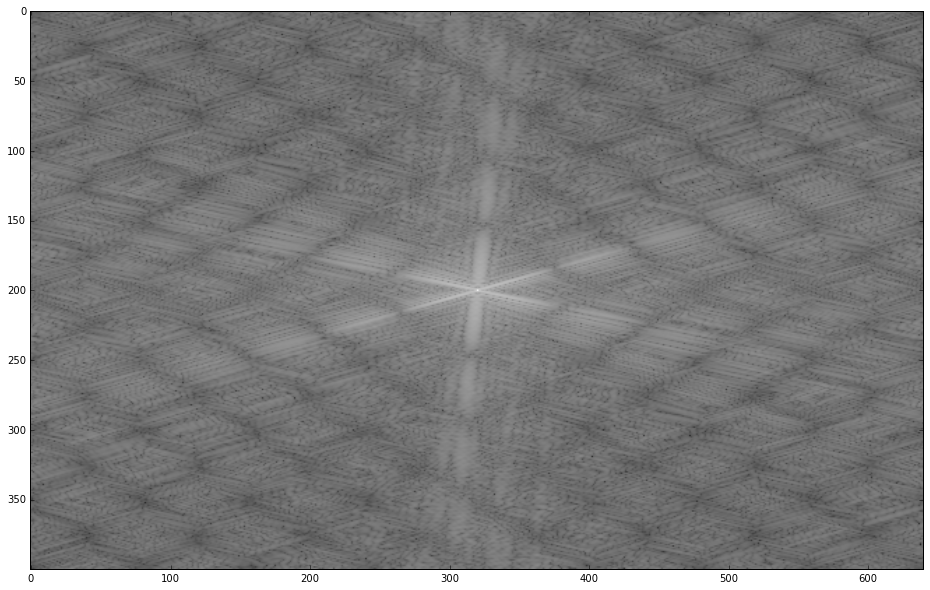
\includegraphics[scale=0.25]{A}
\end{figure}

\justify{
Why is a B classified as an S? Again examining the result feature by feature.
Considering the box feature: A lies in the region of the V cluster with respect to the box feature axis.
This can also be explained by the diagonal lines $u = v$ and $u = -v$ in Fourier space of B as seen in figure 9. These have lower magnitude
than the letter A, and as a result have a lower value in the box feature axis. Secondly,
examining the classification based on the vertical rectangle feature:
the vertical rectangle feature is sensitive to horizontal change. Examining the Fourier space for B,
we can see a vertical line of relatively high magnitude running through the center, this corresponds to
the three horizontal sections partly composing the character B. As a result of this, the vertical rectangle feature
classifies this as a T. Therefore, similarly to A -  because of the combination of the fact that the B is classified
as a T by the vertical rectangle feature, and as a V by the box feature, the result is the the B is also classified as
an S.
}

\begin{figure}[h!]
  \caption{Fourier space of  B}
  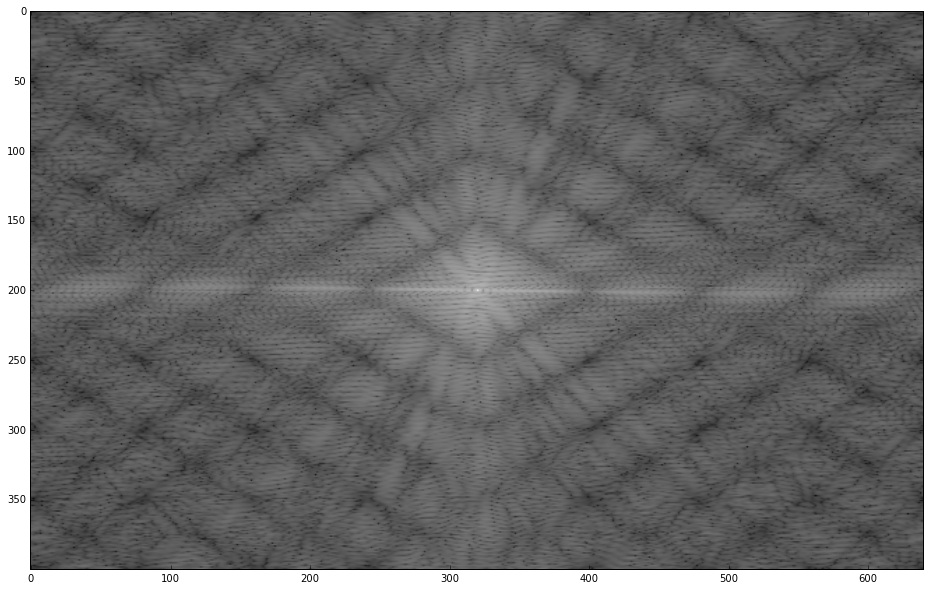
\includegraphics[scale=0.25]{B}
\end{figure}

\end{flushleft}



\end{document}
